\documentclass[]{article}

\usepackage{amsmath}
\usepackage[]{graphicx}
\usepackage{subfigure}
\usepackage[latin1]{inputenc}
\usepackage{comment}
\usepackage{url}
%\usepackage{biblatex} 
%\usepackage[pdftex]{graphicx}
\usepackage{anysize}

\providecommand{\e}[1]{\ensuremath{\times 10^{#1}}}

\marginsize{3cm}{3cm}{2cm}{2.5cm}%l r t b

\title{Gaze Enhanced Speech Recognition for Truly Hands-Free and Efficient Text Input During HCI}
 
\author{Matheus Portela}
\author{David Rozado}

\author{
  Matheus Vieira Portela\\
  Mechatronics Engineering Student\\
  University of Brasilia, Brazil\\
  \em{Scholar of CNPQ}\\
  \texttt{matheus.v.portela@gmail.com}\\
  \and
  David Rozado\\
  Postdoctoral Fellow\\
  ICT Centre\\
  CSIRO, Australia\\
  \texttt{David.Rozado@csiro.au}
}

\setlength\parindent{0pt} %no indentation in paragraphs
% Document starts
\begin{document}

\maketitle

\section{Abstract}
Algorithms based on modeling speech as a finite-state hidden Markov process have been the most successful approach used
to solve the automatic speech recognition problem. Nonetheless, the performance of current speech recognition algorithms
is well below that of humans. Error rates of computational speech recognition are an order of magnitude greater than
human speech recognition in quiet environments. Machine performance degrades even further in environments with noise
channel variability and spontaneous speech. Humans can also better recognize sounds with very little high-level
grammatical information. The error rates of current speech recognition systems are frustrating for the humans using
them. In this work, we present an innovative form of correcting misrecognized words during a speech recognition task by
using gaze tracking technology. Specifically, we propose to use the user's gaze to point at misrecognized words during a
speech recognition task and to select appropriate word alternatives also using gaze. We compare  the performance of this
multimodal approach to speech recognition with traditional modalities of correcting misrecognized words: usage of the
mouse and the keyboard and usage of voice alone. The results of the user study show that while the proposed system is
not as fast as using the mouse and the keyboard for correction, gaze enhanced correction remains a truly hands-free
means of interaction with the computer with obvious advantages for certain types of users such as those who lack  motor
mobility or dexterity of the hands or those suffering from repetitive strain injuries. The system is also advantageous
for scenarios that prohibit or discourage the usage of the hands to interact with the computer. The gaze enhanced
correction of misrecognized words also significantly outperforms the other truly hands-free correction modality: voice.
These results evidence the advantages of the proposed gaze enhanced speech recognition modality to improve the speech
recognition experience for a variety of users and scenarios.\\


\textbf{Keywords:} Eye tracking, gaze tracking, gaze aware interfaces, pervasive computing, speech recognition,
multimodal interaction, human computer interaction, HCI, gaze responsive systems 


\section{Introduction}
In computer science, speech recognition refers to the computational translation of spoken words into text.
Using speech to create or edit documents offers the potential to be a faster and more natural way to interact
with computers as well as a hands-free modality of Human Computer Interaction (HCI) with obvious positive implications
for handicapped users or scenarios where computer users have their hands engaged in other tasks, for example surgeons in
the operating room.


Although there has been a significant increase in the accuracy performance of speech recognition software over time,
error rates still make the technology cumbersome to use for everyday interaction and functional speech recognition still
requires a relatively long learning curve on the part of the user to properly master it. Still, misrecognized words
occur often during speech recognition tasks even for advance users. For instance, previous works have shown that several
factors increase the error rates in conversational speech: infrequent words, very fast or very slow speech, and long
words among others \cite{Goldwater2010181}.


The correction of speech recognition errors or misrecognized words can be carried out manually with a traditional
keyboard and mouse to select the misrecognized word and retype it, which is probably the most widely used method for the task. This modality can
be perfectly valid for some scenarios, but it is not truly hands-free anymore.


The usage of voice for correction of misrecognized words during speech recognition maintains the notion of exclusively
hands-free input to the computer. In practice however, this modality can be very frustrating for the user since
``certain" challenging words are extremely difficult to be properly recognized by speech recognition engines. Hence,
this correction modality is extremely error-prone and frustrating for users considering the user has to first select by voice
the wrong word, then repeat over and over again the right word until it is properly recognized, and then choosing it
from a list of similar alternatives. As all of this has to be done by voice, errors are frequent. Users with a
foreign accent struggle markedly with this form of interaction. Furthermore, repeating several times the same word makes
the vocal cords go through the same pattern of folding and vibrations repeatedly which has been shown to cause voice
strain \cite{voiceproblems}.

 
In this work, we propose the enhancement of speech recognition software with gaze tracking technology to speed up the
correction of misrecognized words and to maintain speech recognition truly hands-free. A gaze tracking system tracks the
point of regard (PoR) of the user on the screen by monitoring the users pupils while sitting in front of a computer
\cite{Rozado2012a}. With the proposed modality, the user is required to simply gaze at the misrecognized word and then
select the correct word from a gaze dependent emerging panel of most likely alternative words. If the correct
word is not in the panel of alternative words, the user has the chance of trying to utter it again. The correct word is
selected from the panel just by looking at it.


The experimental part of this work compares the three aforementioned modalities of correcting misrecognized words during
 a speech recognition task: usage of the traditional keyboard and mouse, usage of voice and usage of gaze.


To our knowledge, the idea of using gaze to correct misrecognized words in a speech recognition task has not been 
explored before in the research literature. There exists however work on gaze aware systems that use gaze tracking data
to adapt their behavior to the patterns of user's gaze.


The notion of gaze attentive interfaces is neatly explained in \cite{hyrskykari2006eyes}. That work focused on examining
the benefits and limitations of using eye movements in the human computer interface (HCI). Authors tested 
the performance of gaze aware applications and concluded that they had a potential to be more
pleasing and effective than traditional application interfaces.

 
In \cite{Kozma2009}, authors introduced a gaze-based interface for browsing and searching images that refined search
engine prediction results using relevant images obtained by monitoring the user's gaze patterns over the first images
returned by the search engine. The work showed that there was sufficient information in the gaze patterns to complement
or even replace explicit feedback given by the mouse on images of interest.


Authors in \cite{Tourassi2010} explored the potential of a Computationally Aided Diagnostics System (CADS) through
making it context sensitive by providing decision-support to radiologists' focus of attention during visual search
in a mammography analysis task. Their system combined machine learning prediction algorithms to obtain a list of
coordinate places on the image with potentially cancerous tissue to direct the attention of the radiologist towards
those locations


The work from \cite{Koesling2011} studied gaze behavior in a first person shooter game and suggested that game engines
might use this knowledge to anticipate actions that players have not executed yet. Authors provided a convincing
argument that a gaze dependent anticipation module should enhance game character behaviors and make them much "smarter".


The project text 2.0 from \cite{Biedert2010} studies the advanced display of text by monitoring user's gaze during
reading while providing extra features to enhance the reading experience. In this manner, gaze behavior is used to make
text responsive to readers' gaze patterns by, for instance, providing dynamic pop up definition boxes when a user gazes
at a word for an amount of time exceeding a predefined threshold.


Authors in \cite{Hillaire2008} described the usage of focus points to improve the visual effects in virtual environments
by adapting the rendering technique of a 3-D model to a user's gaze position using models of visual attention. This was
done with the intention of improving users' sensations during first person navigation in the 3-D environment.
In a similar work, authors in \cite{Rahardja2009} described a dynamic display system that naturally and interactively
adapts the display properties as the user's eyes move around a high definition panoramic scene.


Gaze has also been used to input text or commands in a variety of scenarios \cite{myiwann2011}. Authors in
\cite{fasthandsfreewritingbygaze} showed an innovative approach for fast text input using gaze named Dasher. Dasher is a
dynamic text input system controlled by gaze that uses a language model to facilitate letter completion and selection
within a word/sentence. Users enter text by tracking the desire character with the eyes, rather than by performing
discreet gestures. Dasher can write up to 25 words per minute (wpm) after considerable familiarization with the system
in comparison to the maximum of 15 wpm for expert users using an on-screen keyboard.
 

Finally, the work from \cite{Pomarjanschi2012} studied the effectiveness of gaze guidance on the visual performance of
drivers. Their system monitors drivers' gaze to provide them with alerts of potential dangers on the road (obstacles,
incoming pedestrians, nearby cars) if the gaze monitoring system determined that the driver is not paying attention to
them. Such a system detects driver's distraction with respect to an incoming pedestrians coming from the right and it
will display an arrow pointing towards the pedestrian in the area of the windshield where the user is paying attention
to.


Once considered pure science fiction, automatic speech recognition (ASR) has been well studied over the past few decades
over various distinguishing perspectives. This includes the acoustic-phonetic approach, pattern recognition approach, knowledge
based approach, connectionist approach, and using support vector machines. Ghai et al. summarizes these various points of view
in their work \cite{GhaiSingh}.


The speaking mode is also an important factor that has to be considered in ASR systems, since its constraints require
different designs. An isolated word speech recognition (IWR) assumes that one single word with well defined beginning
and ending points is being uttered, which imposes great limitations on ASR. In order to deal with several words
separated by pauses, connected word recognition (CWR) should be considered. Continuous speech recognition (CSR) deals
with the scenario where words are connected, i.e., the boundaries of each individual word are unclear, requiring more
sophisticated systems, such as the usage of Hidden Markov Models (HMM) \cite{Young2001}. Finally, there is the main
objective for ASR systems: spontaneous speech recognition - the most natural speech mode. The difficulty here lies on
the various odd sounds humans produce when speaking in a natural fashion, such as when expressing hesitation or
uncertainty \cite{GhaiSingh}.


Even with state-of-the-art approaches to ASR, external noise degrades considerably the quality of the recognition. Gong
\cite{Gong1995261} presents several mathematical approaches that deal exclusively with improving recognition in noisy
situations, specially the most successful technique: speech model compensation. Still in this area of research, Chan et
al. \cite{Chan2001} proposed to use myo-electric signals to refine ASR in extremely noisy environments, with promising
results.


Another aspect that quickly degrades quality of speech recognition is the presence of accent in the user speech. In their work,
Kat and Fung \cite{KatFung758102} employ accent detection and accent-adaptive recognition for Chinese users to transform a native
accent dictionary in an accent-adapted dictionary using as prior information the native language of the speaker. Using this
methodology, the error rate of recognition could drop by up to 13.5\%.


When these variables that rise the recognition error rate are slightly controlled, ASR systems find appropriate niche
applications, specially when integrated with different interaction modalities. Vo and Wood \cite{VoWood550794} present a
multimodal calendar integrating speech, gesture and handwriting recognition systems. The main advantage of multimodal
systems is that the final hypothesis can integrate recognition results from each modality alone and, in the end,
produces a better and more complete recognition. Even though recognition errors can degrade performance, the multimodal
approach counterbalances it.


Tse, Greenberg and Shen \cite{Tse2006} use speech- and gesture-based recognition over digital tables to transform a
previously single-user interaction into a multi-user one. In this exciting research, they enabled well-known commercial
software such as the map-viewer and games to be used simultaneously by many users, where speech was responsible for
command and control interaction (e.g., 'stop' or 'fly to Boston') and gestures could enable selection, zooming or
dragging, for instance.


In summary, we present here a multimodal approach to HCI that augments speech recognition with a gaze attentive
interface for correction of misrecognized words. This approach offers the advantage to maintaining a truly hands-free
paradigm of inputting text into a computer. To obtain empirical validation to our hypotheses, we explore through a
comprehensive user study how this multimodal paradigm compares to the two traditional modalities used to correct
misrecognized words, using voice alone and using the mouse and the keyboard, in terms time, task completion rate, and
physical effort required to complete the task.


\section{Methodology}
The goal of the user study was to compare the correction of misrecognized text using the gaze-based correction method
with the voice and mouse and keyboard correction methods in a previously not trained ASR system. For this purpose, a graphical user interface (GUI) was
designed and implemented to be shown to the subjects for each one of the correction modalities. The video at
\url{http://www.youtube.com/watch?v=xdBoNsMthr8} provides a good overview of the experimental setup and the different
correction modalities being compared in the user study. We encourage the interested reader to view the video in order to
gain a good understanding of the work presented here.


\subsection{Eye Tracking}
Eyes are used by humans to obtain information about the surroundings and to communicate information. When something
attracts our attention, we position our gaze on it, thus performing a \textit{fixation}. A fixation usually has a
duration of at least 150 milliseconds (ms). The fast eye movements that occur between fixations are known as
\textit{saccades}, and they are used to reposition the eye so that the object of interest is projected onto the fovea.
The direction of gaze thus reflects the focus of \textit{attention} and also provides an indirect hint for
\textit{intention} \cite{velichkovsky}.


A video-based gaze tracking system seeks to find where a person is looking, i.e. the Point of Regard (PoR), using images
obtained from the eye by one or more cameras. Most systems employ infrared illumination that is invisible to the human
eye and hence it is not distracting for the user. Infrared light improves image contrast and produces a reflection on
the cornea, known as corneal reflection or glint. Eye features such as the corneal reflections and the center of the
pupil/iris can be used to estimate the PoR. Figure \ref{screenGazeTracker} shows a screenshot of an eye being tracked by
the open-source ITU Gaze Tracker \cite{lowcostitugazetracker,Rozado2012}. In this case, the center of the pupil and two
corneal reflections are the features being tracked.


\begin{figure}[ht]
\begin{center}
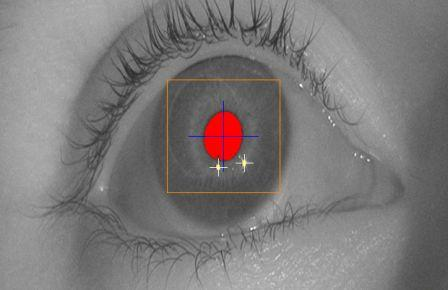
\includegraphics[width=0.5\textwidth, height=40mm]{figures/screenGazeTracker.jpg}
\vspace{-3mm}
\end{center}
\caption{\textbf{The Open Source ITU Gaze Tracker Tracking One Eye.} The
features tracked in the image are the pupil center and two corneal reflections. These features are used by the gaze 
estimation algorithms to determinine the PoR of the user on the screen.}
\label{screenGazeTracker}
\end{figure}


\subsection{Speech Recognition}
Speech is one of the most natural communication skills. Humans use the vocal tracts to produce sounds, the air as a
communication channel, and the auditory system as a pass-band for frequencies in the 0-20kHz spectrum. The basic unit of
speech are the \textit{phonemes} which, when sequenced, are decoded as words by another person. However, the
pronunciation of phonemes leads to \textit{coarticulation}, i.e., to utter them without an intervening pause, which
affects the neighbor phonemes in several ways \cite{Douglas2008}.


In order to perform recognition, many pattern recognition techniques have been employed. When words are uttered, Hidden
Markov Models (HMM) compare the collected data to a set of probabilistic density functions (PDFs) of \textit{acoustic
models} and select the one with highest probability. Afterwards, the result is integrated to \textit{language models}, which
incorporates syntax and semantics to ASR \cite{Douglas2008}.


\subsection{Participants}
Nineteen participants took part in the user study. Among them, there were 10 native English speakers and 9 non-native
English speakers (17 male and 2 female). This is mentioned to account for the fact that speech recognition performance
varies significantly between native and non-native speakers.


\subsection{Apparatus}
The experiment used a GUI interface written in Python 2.6 using the Qt 4.8.4 Framework, by Digia, and the PyQt 4.9.6
bindings. The speech recognition system incorporated in the interface was provided by the Microsoft Speech Application
Programming Interface (SAPI), using version 5.1 of the SDK, in the Windows 7 operational system. In order to track
the gaze, a Tobii X1 Gaze Tracker was used together with the Tobii SDK 3.0 RC1 for Windows.


\subsection{Experimental task}
Each participant was requested to dictate 10 sentences with an allotted time of 60 seconds per sentence.
This task was repeated three times, one for each correction modality: gaze, voice and mouse and keyboard making a total
of 30 dictated sentences for each subject. The sentences and the correction modality were randomly shuffled between
experimental trials in order to smooth out ordering effects on the correction modalities performance. Previously to the
beginning of each experimental trial, we ran a few test trials of each correction modality to make the
subject comfortable with the interface. Also, a new empty Windows speech recognition profile was created for each subject
in order to avoid the previous trials to facilitate recognition of the sentences.


The user interface, displayed in Figure \ref{guiExampleEdited} shows the correction modality, the target sentence and
the number of the trial (from 1 to 30), on the top of the screen. When a speech utterance was recognized by the ASR, the
words would be presented on the center of the screen. These words could be corrected in three different ways, determined
by the correction modality:
\begin{itemize}
  \item Mouse and keyboard: When clicking on a word with the mouse, a correction panel would pop up showing a list
  of at most 5 alternative words, which could also be selected by clicking. When the desired word was not presented as
  an alternative, clicking again on the word would generate a line edit and allow the subject to type the desired word with the keyboard;
  \item Voice: A correction panel was raised by saying the command ``correct" followed by the
  desired word to correct. In this mode, alternative words presented in the correction panel are preceded by a number that, when pronounced,
  selects the corresponding word. When the desired correction was not presented in the correction panel, pronouncing
  again the word would refresh the menu with a new list of best-guess alternatives produced by the speech recognition engine.
  \item Gaze: Fixating on a word with gaze for a dwell time of 2 seconds would pop-up correction panel with the list of 
  at most 5 alternative words. Similarly, the alternative word could be selected by fixating the gaze for 2 seconds over it.
  Pronouncing the word again would refresh the menu with new alternatives.
\end{itemize}


\begin{figure}[ht]
\begin{center}
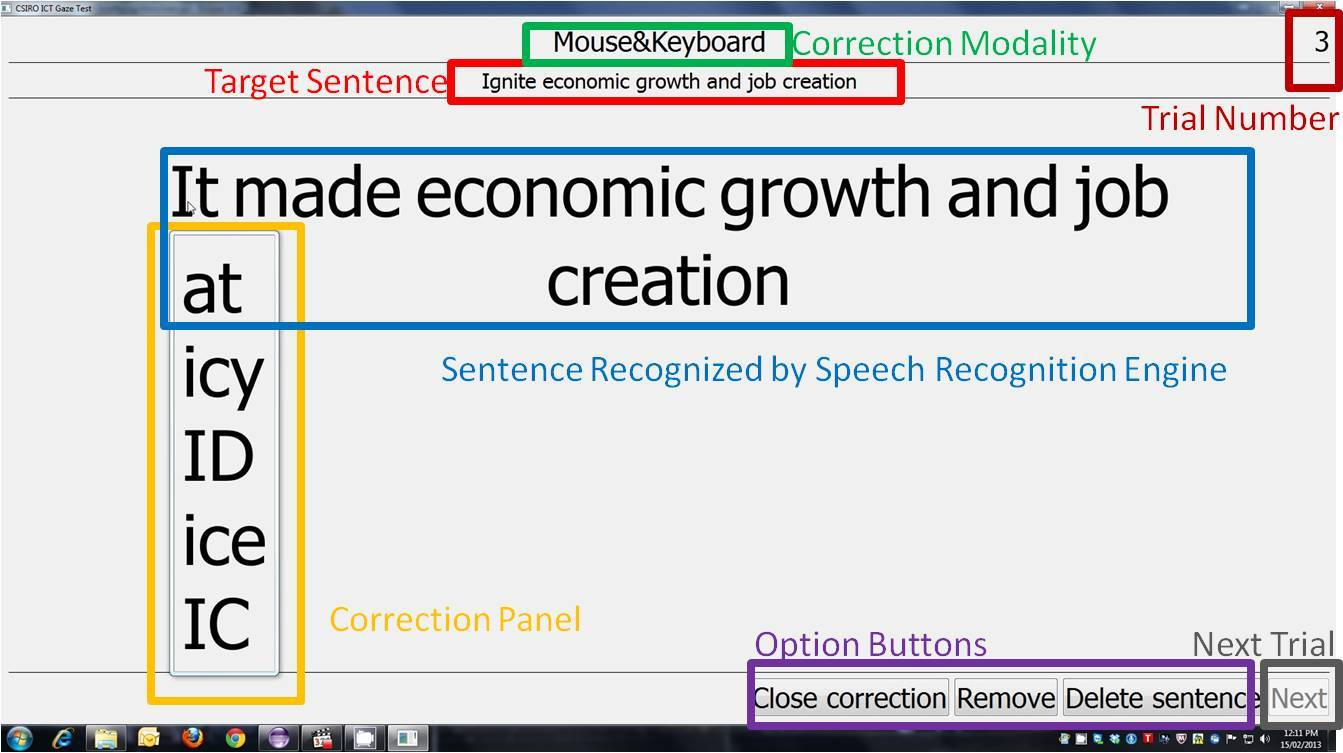
\includegraphics[width=0.75\textwidth]{figures/guiExampleEdited.jpg}
\end{center}
\caption{\textbf{GUI Used in the Experiments.} This figure shows highlighted in different colors the different parts 
composing the user interface exposed to the subjects while participating in the user study.}
\label{guiExampleEdited}
\end{figure}


On the bottom of the screen, three options buttons were available when a word was being corrected, i.e., with the
correction panel opened: ``Close correction", which would close the correction panel menu of alternative words to
substitute a misrecognized word, ``Remove", that would delete the word, and ``Delete sentence", which would delete the
entire recognized sentence. A ``Next" button would become active when the recognized sentence matched the target
sentence or when the allotted time of 60 seconds had been excedeed. When the user had correctly pronounced the desired
sentence, the ``Next" button and the target sentence would become green to indicate that the user could go to the next
trial. However, if the desired sentence was not reached in less than 60 seconds, the ``Next" button and the target
sentence would become red, indicating that the user has failed to correct the sentence in suitable time and could
proceed to the next trial. All these buttons could be activated either by using the mouse or the active correction
modality.

At the end of the experiments, the subjects involved in the user study were required to fill a questionnaire asking them
about their subjective experience with the different correction modalities.


\subsection{Measures}
During the experiment, time to complete the task was measured.  Timing would stop when the active sentence being uttered
and edited matched the target sentence or if the user failed to achieve the target sentence within the allotted 60
seconds threshold. When correcting by mouse and keyboard, the mouse displacement and number of keystrokes presses were
recorded. Each sentence also was marked indicating whether the trial has failed or not.


Furthermore, both the pronounced and the target sentence were recorded, this data was later used to calculate the Damerau-Levenshtein
distance \cite{Damerau1964} between them. This distance reveals how far two strings are from each other considering four
basic operations: insertion, deletion, substitution of a single character, and transposition of two adjacent characters.

Lastly, the user questionnaire was composed by the following five questions, where the subjects were able to answer
either ``Traditional keyboard and mouse", ``Voice" or ``Gaze".


\begin{itemize}
  \item Which method do you find fastest to correct misrecognized words during speech recognition?
	\item Which method do you find the least error prone to correct misrecognized words during speech recognition?
	\item Which method do you find the more fatiguing to get the job done?
	\item Which method would you prefer to use to correct misrecognized words during speech recognition?
	\item If you could not use your hands during HCI, which method would you prefer to use to correct misrecognized words during speech recognition?
\end{itemize}


\section{Results}
The average time of each experimental trial to achieve the target sentence using a given correction modality is
displayed in Figure \ref{timeFig}. A Levenes' test for equal variance for the 3 correction modalities failed ($p=2.1$).
Hence, the results of the ANOVA analysis need to be interpreted with caution. The F-test produced a value of
$F(2,54)=17.43$, $p=1.44\e{-06}$. A Posthoc Bonferroni-Holm test indicated significant differences between the
voice-mouse\&keyboard, gaze-mouse\&keyboard and gaze-voice modalities with $p=4.24\e{-06}$, $p=3.6\e{-05}$ and $p=0.02$,
respectively.
 

\begin{figure}[!ht]
\begin{center}
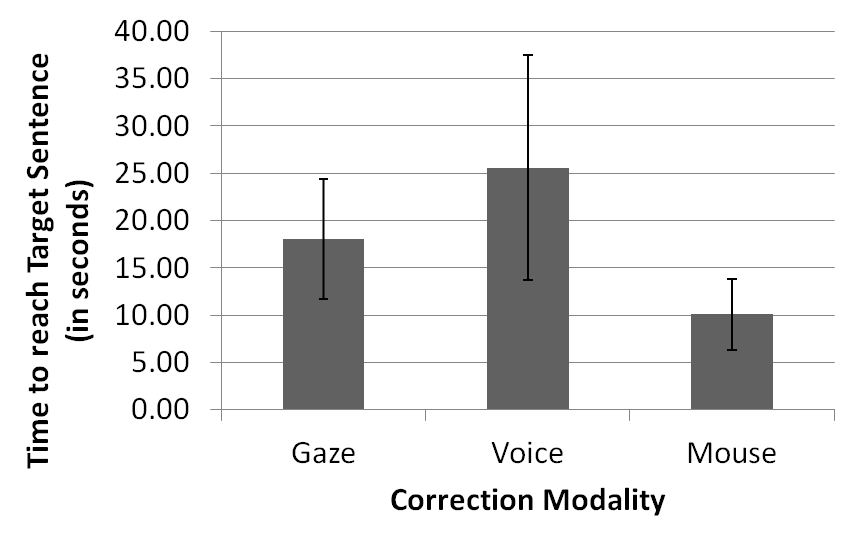
\includegraphics[width=0.9\textwidth,height=65mm]{figures/time.png}
\end{center}
\vspace{-3mm}
\caption{\textbf{Average Time Required to Achieve Target Sentence.} The figure displays the average time per trial that
the speech recognition engine with different correction modalities required to reach the target sentence.}
\label{timeFig}
\end{figure}


Figure \ref{mouseDisplacement} shows the average displacement in pixels of the mouse during each experimental trial for
each correction modality. Again, a Levene's test failed to find equal variance among experimental conditions. The ANOVA
analysis showed significant differences between groups,  $F(2,54)=25.06$, $p=2.0\e{-08}$. A Posthoc Bonferroni-Holm test
found significant differences between the gaze-mouse\&keyboard and voice-mouse\&keyboard modalities,  $p=1.48\e{-05}$,
$p=1.48\e{-05}$ respectively.


\begin{figure}[!ht]
\begin{center}
\vspace{-3mm}
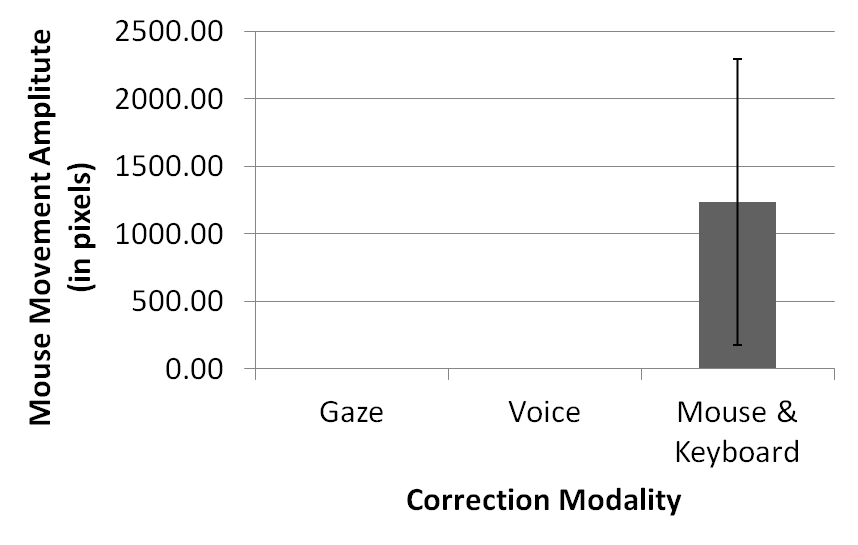
\includegraphics[width=0.9\textwidth,height=65mm]{figures/mouseDisplacement.png}
\end{center}
\caption{\textbf{Average Mouse Movement Amplitude Required to Complete the Task.} The figure displays the average mouse
movement amplitude in pixels per trial required by each correction modality to reach the target sentence during the
experimental trials.}
\label{mouseDisplacement}
\end{figure}


The average number of keystrokes required from the subjects to achieve the target sentence by each correction modality
during the experimental trials is shown in Figure \ref{keystrokes}. Again a Levene's test failed to assume equal
variance. The ANOVA analysis showed statistically significant differences between the results of the
difference correction modalities, $F(2,54)=36.79$, $p=8.29\e{-11}$. 


\begin{figure}[!ht]
\begin{center}
\vspace{-3mm}
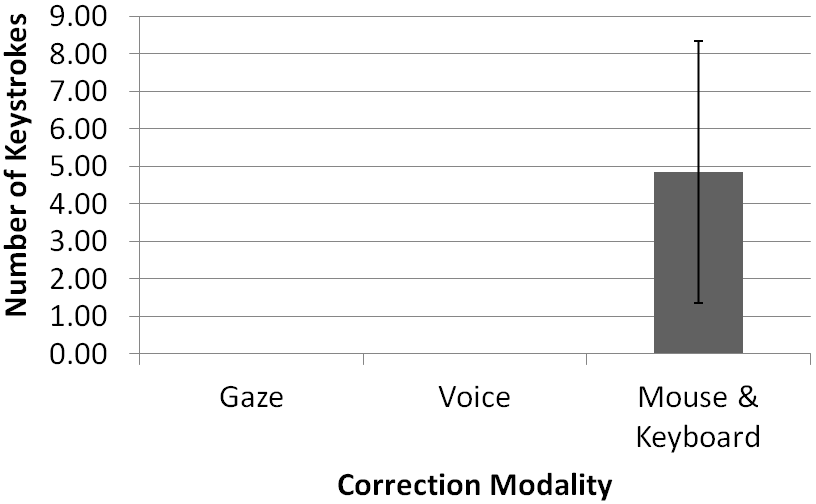
\includegraphics[width=0.9\textwidth,height=65mm]{figures/keystrokes.png}
\end{center}
\caption{\textbf{Number of Keystrokes Required to Complete the Task.} The figure displays the average number of
keystrokes presses required by each correction modality to reach the target sentence
during the experimental trials.}
\label{keystrokes}
\end{figure}


Figure \ref{failFig} shows the average number of trials in which the user was unable to reach the target sentence in the
allotted time of 60 seconds using the given correction modality. The Levene's test also failed to determine equal
variance. The ANOVA analysis showed statistically significant differences between the results of the
difference correction modalities, $F(2,54)=17.92$, $p=1.07\e{-06}$.   A Posthoc Bonferroni-Holm test found
significant differences between the voice-mouse\&keyboard modalities, $p=6.62\e{-06}$, gaze-mouse\&keyboard modalities
$p=9.23\e{-05}$ and gaze-voice modalities $p=4.02\e{-03}$.


\begin{figure}[!ht]
\begin{center}
\vspace{-3mm}
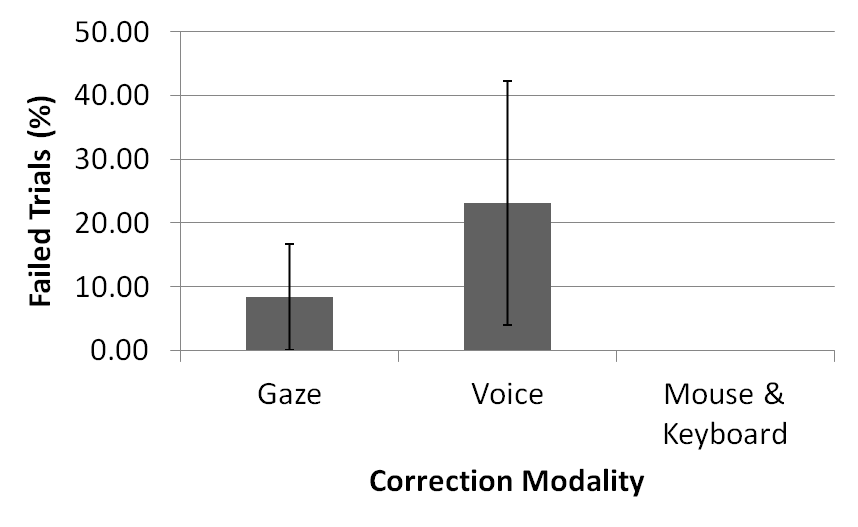
\includegraphics[width=0.9\textwidth,height=65mm]{figures/fail.png}
\end{center}
\caption{\textbf{Number of Failed Trials.} The figure displays the percentage of trials in which the user
was unable to reach the given target sentence within the allotted time of 60 seconds.}
\label{failFig}
\end{figure}


The average Damerau-Levenshtein distance between the target sentence and the generated sentence within the 60 seconds
time window for each correction modality is shown in Figure \ref{dldistance}. The ANOVA analysis generated statistically
significant differences between modalities with values $F(2,54)=11.60$, $p=6.44\e{-05}$. A Posthoc Bonferroni-Holm test
found significant differences between the voice-mouse\&keyboard modalities, $p=5.18\e{-04}$, gaze-voice modalities
$p=4.44\e{-03}$ and gaze-mouse\&keyboard modalities $p=1.71\e{-02}$.


\begin{figure}[!ht]
\begin{center}
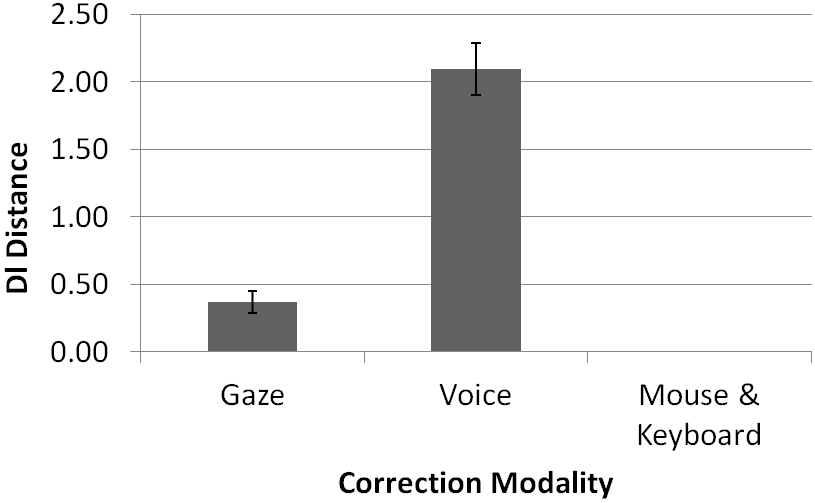
\includegraphics[width=0.9\textwidth,height=65mm]{figures/dldistance.png}
\end{center}
\caption{\textbf{Damerau-Levenshtein Distance.} This figure shows the average Damerau-Levenshtein distance per
trial between the target sentence and the generated sentence for the different correction modalities.}
\label{dldistance}
\end{figure}


Subjects involved in the user study  expressed their subjective impressions about the different correction
modalities being compared through a user questionnaire, the results of which are visible in Figure \ref{questionnaire}.


\begin{figure}[!ht]
\begin{center}
\vspace{-3mm}
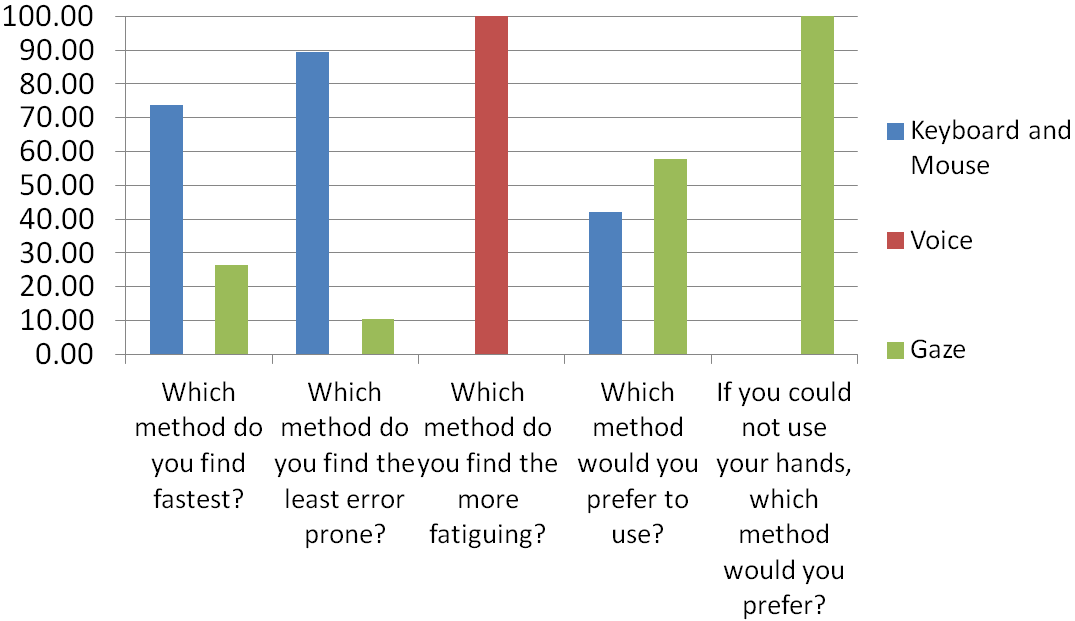
\includegraphics[width=0.95\textwidth,height=65mm]{figures/questionnaire.png}
\end{center}
\caption{\textbf{User Questionnaire.} Subjective opinions expressed by the subjects that participated in the user
study about their perceptions of the different modalities being compared to correct misrecognized words.}
\label{questionnaire}
\end{figure}


\section{Discussion}
The results of the user study showed that the gaze enhanced correction modality for a speech recognition task is not as
fast as using the mouse and the keyboard for correcting misrecognized words. Yet, the gaze based correction modality is
significantly faster than using voice alone for correction and it is truly hand-free as opposed to the Mouse\&Keyboard
modality that required the usage of the hands for correction of misrecognized words. The time performance of the gaze enhanced speech
recognition can be improved in future research by implementing more sophisticated selection methods, replacing the 2
seconds fixation used in this work, by for instance dynamic and continuous selection of words just by looking at them. 
This alone would most likely improve the speed performance of the gaze correction modality.


The amount of mouse movement displacement required to achieve the target sentence was obviously non-existent for the
gaze and voice correction modalities due to their true hands-free nature. The same can be say of the amount of
keystrokes presses required for correction of misrecognized words. The gaze and voice correction modalities are
obviously advantageous in this regard, since they completely eliminate the need of the physical effort associated to
mouse movements and keystrokes presses. This is particularly beneficial for users with limited or no movement control of
the hands, limited dexterity, users suffering from repetitive strain injury (RSI) and for scenarios that prohibit or
discourage hand-based interaction. Voice correction of misrecognized words however, can easily lead to voice strain.
This is due to the accuracy limitations of speech recognition algorithms that make it necessary for the users to repeat
several times voice commands and utterance of the target word until the appropriate word is properly situated into its
target position within the text. Gaze-based correction, on the other hand, does not suffer from any of the previously
mentioned drawbacks of the alternative modalities.


In terms of the number of failures registered during the experimental trials to achieve the target sentence, the gaze
modality was significantly better at reaching the target sentence than the voice modality but worse than the mouse \&
keyboard modality. This was also evident in the Damerau-Levenshtein distance between the target sentence and the
achieved sentence during the experimental trials. Here, it is important to emphasize that the most of the subjects
involved in the user study had never been exposed to gaze tracking technology before. Hence, they did not have time to
properly familiarize themselves with the technology. Given enough time to go through the learning curve of using gaze
interaction would most likely allow learning effects to take place and improve the performance of the gaze based
correction modality.


The main limitation of the proposed modality is due to the constraints in gaze accuracy that any gaze estimation
algorithm  has. Using the proposed system with the typical font size that average users employ for editing texts would
be challenging since it would be difficult for the system to discern the particular word at which the user is gazing
at. Hence, in our user studies we employed relatively large font sizes. Algorithms that would respond to gaze behavior
in a context aware manner could aid in disambiguating where the user is intending to point to. This could be done by
opening the correction panel in the word nearest to the gaze position with the least amount of confidence in the
recognition results. Innovative dynamic displays of alternative words could also help in this regard.


In conclusion, the gaze modality for correction of misrecognized words is not as efficient in terms of accuracy and time
to completion as the traditional mouse \& keyboard modality but it possesses the advantage of being truly hand-free with
obvious  implications for handicapped computer users, users suffering from RSI syndrome and for scenarios where the
usage of the hands is not possible (surgery room for instance). Moreover, the gaze modality significantly outperforms
the other hand-free modality to correct misrecognized words, using voice, in all the variable being monitored in the
user study. Furthermore, the gaze based correction modality also prevents the appearance of voice strain for the
correction of misrecognized words since it prevents considerably the amount of of utterances required to correct a word.


In light of the evidence presented here, we assert the advantages of the proposed multimodal approach to HCI that
complements speech recognition with gaze tracking and gaze interaction to create a truly hands-free multimodal interface
for speech recognition tasks that is faster and more accurate than using voice alone to correct misrecognized words
while remaining a truly hands-free form of interaction.


\bibliographystyle{ieeetr}
\bibliography{library}

\end{document}
